\documentclass[11pt]{article}
%Gummi|065|=)
\usepackage[linesnumbered,ruled,vlined]{algorithm2e}
\usepackage{xcolor}
\usepackage[utf8]{inputenc}
\usepackage{amsmath}
\usepackage{amssymb}
\usepackage{changepage}
\usepackage{graphicx}
\usepackage{hyperref}
\usepackage{listings}
\usepackage{xcolor}
\usepackage[english]{babel}
\definecolor{codegreen}{rgb}{0,0.6,0}
\definecolor{codegray}{rgb}{0.5,0.5,0.5}
\definecolor{codepurple}{rgb}{0.58,0,0.82}
\definecolor{backcolour}{rgb}{0.95,0.95,0.92}

\lstdefinestyle{mystyle}{
    backgroundcolor=\color{backcolour},   
    commentstyle=\color{codegreen},
    keywordstyle=\color{magenta},
    numberstyle=\tiny\color{codegray},
    stringstyle=\color{codepurple},
    basicstyle=\ttfamily\footnotesize,
    breakatwhitespace=false,         
    breaklines=true,                 
    captionpos=b,                    
    keepspaces=true,                 
    numbers=left,                    
    numbersep=5pt,                  
    showspaces=false,                
    showstringspaces=false,
    showtabs=false,                  
    tabsize=2
}

\lstset{style=mystyle}
\title{\textbf{Internship report}}
\author{Nicolas YAX}
\date{}
\begin{document}

\maketitle
M1 student - ENS Paris Saclay - Adrien Doerig - Tim Kietzmann
\section{Context}
\subsection{Global scientific context}
Nowadays image processing technologies can be found everywhere starting from smile recognition in your camera to massive automatic surveillance in China. The problem of image classification is well known and efficiently solved in most engineering applications. However those algorithms still aren't perfect and features such as adversarial examples appear. Adversarial examples can be a real issue as for automatic cars that could be wronged by panels put in specific locations that will try to fool the algorithm to generate dangerous behaviour from the car. Those features exist because of the distance between models and biological computation. We hope that by changing the model to something closer to realistic computation those features might disapear or at least be less impactfull.
To understand this state of the art project we will need to see a lot of basic necessary knowledge about machine learning starting from neural networks until BL and BLT networks without forgetting reinforcement learning state of the art methods, recurrent networks and convolutions.
\paragraph{Neural Networks}
Probably the most famous data structure used in Machine Learning neural networks are a crucial part of this project. A neural network is a function from $\mathbb{R}^m$ to $\mathbb{R}^p$ with $n$ parameters $(w_1,...,w_n)$. Its structure is a tradeoff between neural biological computation and computational effectiveness. 
\newpage
\begin{figure}[h]
\centering
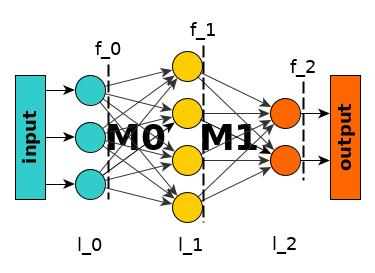
\includegraphics[scale=0.40]{layers.jpg}
\caption{Small neural network with its layers $(l_0,l_1,l_2)$, its matrix $(M_0,M_1)$ and its activation functions $(f_0,f_1,f_2)$. Bias aren't represented for the sake of clarity.}
\label{layers}
\end{figure}

The global structure of brain relies on layers of neurones to process information deeper and deeper into more complex representations \ref{layers}. This structure is approximated by the use of matrix to spread the state of a layer to the next one : \\

with $l_{i}$ the $i^{th}$ layer ($i\le q$), $M_i$ the matrix to compute the excitatory signal leaving layer $l_{i}$ toward layer $l_{i+1}$, $f_i$ the activation function of layer $l_i$ (compute the activation of neurones from the excitatory signal) and $b_i$ is a bias.
\begin{equation*}
\begin{cases}
l_{i+1} = f_{i}(M_{i}. l_i + b_{i}) \\
l_0 = input \\
l_{q} = output
\end{cases}
\end{equation*}
The whole function is then $$out = f_q(M_q. ... f_i(M_i. ... f_0(M_0.input+b_0) ... + b_i) ... +b_q)$$. Parameters are matrix's weights and biases. They represent connection's strenght between neurones and treshold to excitate neurones. We'll see in next paragraph how to tune parameters to learn something to the neural network.

\paragraph{Supervised Learning}
The supervised learning problem is fairly simple : Starting from a training base $((x_0,y_0),(x_1,y_1), ... , (x_s,y_s))$ we want the data structure (here the neural network) to fit on those values. This means that our model $f$ will verify $\forall i\le s, f(x_i) = y_i$ or at least $f(x_i) \approx y_i$. In practice the first case is almost impossible to reach and we try to minimize a \emph{loss function} that will define the '$\approx$' semantics. The simplest loss function is probably the squared L2 norm : $L = \sum_{i\le s}(f(x_i)-y_i)^2$. 
To minimize this loss with a neural network we can compute the gradient of this norm for each parameter of the network and apply the gradient descent algorithm.
Gradient descent step :
$$\forall i\le n, w_i = w_i - \lambda  \frac{\partial L}{\partial w_i}$$
$$ \mbox{\emph{learning rate}} : 0<\lambda<1$$

If the gradient for a parameter $w$ is positive it means that the loss function should increase as the parameter increases. Thus by decreasing the value of this parameter the loss will decrease and the model will better fit the base. If it's negative the loss should decrease as the parameter increases.
By applying several steps of this algorithm it's possible for a neural network to approximate a base with a pretty good accuracy (L very low).

Defining the loss function is crucial as it will define how the model will fit on a specific part of the base (it's possible to use a weighted loss for example) as well as adding other terms to encourage other properties such as small weights in the network : $L_{small weights} = \sum_{i\le n}|{w_i}|$. Moreover it will also define the way gradients will be optimized which makes it one of the most important thing to work on in machine learning.

\paragraph{Reinforcement Learning}

An other paradigm of machine learning is reinforcement learning. This part of machine learning is very close to the behaviourism theory in psychology. It involves an agent / environment system where the agent will have to learn to behave in order to maximize a reward.
\newpage

\begin{figure}[!h]
\centering
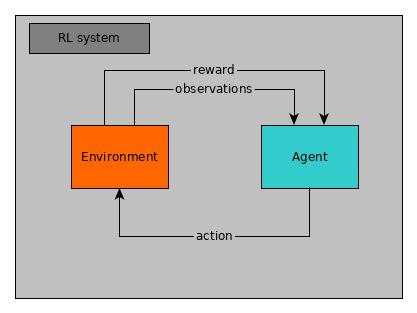
\includegraphics[scale=0.40]{rl.jpg}
\caption{RL system : the agent will see its environment (collect observations) and learn to react to it (chose action) in order to get the highest cumulated reward}
\label{rl}
\end{figure} 
Here is a scheme about RL systems \ref{rl} .

More formally the environment contains a set of states $S$, a set of initial states $S_I\in S$, a set of final states $S_f \in S$, a finite set of actions that can be taken in any state $A$, a stochastic transition function $P$:($S$,$A$)$\rightarrow$($[0,1]^S$) returning a probability distribution over states $S$ when taking an action $A$ in state $S$ in which state $S'$ the environment goes and a reward function $r$:($S$,$A$)$\rightarrow\mathbb{R}$ telling which reward is associated with a transition. This is part of the environment, the agent doesn't know $S$,$A$,$P$ nor $r$.

Now let's see what the agent has. Initially the agent is thrown in the environment with 0 knowledge about it and it will have to explore to learn where best rewards are and which trajectories in $P$ are the most interesting ones. It will have a memory $M$ that will be modelised as the set of previous trajectories. The agent behaviour will be modelised by a function $\pi$:$(S,M)\rightarrow [0,1]^A$ called the \emph{policy} associating a probability distribution over the action space to each state. This function will learn during training.

Each step, the agent is in a state $S_i$ and chooses an action $A_{i} = \pi(S_i\|M+(S_0,...,S_{i-1}))$ which changes its state to $S_{i+1}=T(S_i,A_i)$ and returns the reward $r_i$= $r$($S_i$,$A_i$). If the new state is final, the trajectory is over, if it's not, the agent continues to step. Initialy the agents starts in an initial state $S_0$ (chosen arbitrarily of randomly) and steps. Theoritically speaking trajectories might be infinite but in practice they aren't. Thus a trajectory will be a sequence $\tau$ = (($S_0$,$A_0$,$r_0$),...,($S_i$,$A_i$,$r_i$),...,($S_t$,$A_t$,$r_t$)).

If all trajectories are finite we can easily define the total reward over the trajectory (also known as the \emph{return}): $$ R_{\pi}(\tau)= \sum_{(S_i,A_i,r_i)\in\tau}r_i$$
However in practice trajectories might be very long and only the reward neighbourhood is really interesting. That's why in practice people use a \emph{discount factor} $\gamma$:
$$ R_{\pi}(\tau) = \sum_{(S_i,A_i,r_i)\in\tau}\gamma^{i}.r_i $$
with $\gamma\in]0,1[$ and $l$ the lenght of $\tau$.

To improve the agent will run several trajectories always trying to understand better its environment and finding the best policy to optimize its gain. After each trajectory $\pi$ might be updated by the RL algorithm for this purpose.

The aim of RL is to find the best algorithm to maximize the sum of gain only giving the agent a specified period of time to improve. In practice it could be a robot trying to find a path in ruins of a collapsed building to find survivors. It needs to quickly understand the shape of the environment to map the environment and avoid getting hurt. This means there is a dilemn in RL : exploring of exploiting what the agent already knows. If it explores all the time it won't be able to get enough reward especially if time is short whereas if it explores a bit and after only exploits it knowledge without learning more it may get far less reward than it could.

%Not sure about this. People from my university really like this way to explain problems but it might be an incorrect formulation (which is worst than not putting it)-----
Here is the formal RL Problem : 
\begin{equation*}
\begin{cases}
\mbox{DATA : number of steps $N_s$, return function $R$}\\
\mbox{QUESTION : RL algorithm to get the best cumulated reward $r_c$}
\end{cases}
\end{equation*}
%-----

People usually use a number of steps instead of a number of whole trajectories because trajectories length might vary a lot from one to another.
In practice it's almost impossible to get a complete understanding of the environment (think about Chess and Go which are too complex games with too many states / actions to be fully explored). This means the policy needs to extrapolate its knowledge understanding a logics behind the environment. This can be acheived using structures such as Neural Networks. There are many ways to optimize $\pi$ function but to make it short we will only explore the Policy Gradient method.

In practice observation space and action space are arrays of float values.

In RL there are 2 additional usefull functions that will be used later : $Q$ and $V$. 
$$\forall s\in S, Q_\pi(s,a)=\mathbb{E}_{\tau\|\tau[0]=(s,a,\_)}(R_\pi(\tau)) $$
$$\forall (s,a)\in S\times A, V_\pi(s)=\mathbb{E}_{\tau\|\tau[0]=(s,\_,\_)}(R_\pi(\tau)) $$
$Q_\pi$ represents the value of an action in a specific state after taking this action with policy $\pi$ whereas V represents the value of a state while following $\pi$. We then finaly define optimal $V$ and $Q$ :
$$\forall s\in S,V_*(s) = max_\pi V_\pi(s)$$
$$\forall (s,a)\in S\times A,Q_*(s,a) = max_\pi Q_\pi(s,a)$$

\subparagraph{Policy Gradient and REINFORCE}
The philosophy of the policy gradient method is to see the policy $\pi$ as a function that will be learnt by supervised learning on batches of observations.  The aim of policy gradient is to use a neural network as policy model and to use a specific loss function to increase the score of the agent. This policy will have a probability of chosing a random action as exploration parameter instead of returning its estimated best action.

Usually the algorithm will proceed in 2 phases : first it will collect information from the environment (n trajectories) and then it will fit the policy on those collected data. The policy will be modelised by a neural network which will, given an observation (a vector), return the associated action (a vector).

REINFORCE is probably the simplest Policy Gradient algorithm and is directly using the sum of the estimated expectation over the batch of collected data as loss for the neural network.
$$-\mathbb{E}(\sum_{\tau}R_{\pi}(\tau))$$
The algorithm collects a batch of X trajectories to fit the neural network on it. This process is repeated several time until convergence.
% I don't know if I explain in depth why it's easily computable and independant from P because it might be a lot of math but it helps understanding how it works
This function can be easily computed in practice as well as its gradient. This process of collecting / fitting is repeated several times.
\subparagraph{PPO}
PPO is a state of the art Policy Gradient algorithm designed by OPENAI. It aims at improving REINFORCE by adding few features in the loss function. First when using an algorithm such as REINFORCE, the policy might change too much when fitting. Let's assume the environment is divided into several phases (summer,automn,winter,spring for example) where results of actions could be very different from a phase to another. This kind of learning might result in a policy that would change too much and overfit on each phase, forgetting everything learnt during the previous phase. There is no perfect solution for this issue.

PPO adds a term in the loss that will try to not move too much from the previous policy in order to avoid such a behaviour. This term uses a more complex structure than REINFORCE. The policy will be composed of 2 neural networks : the policy network which returns actions and the value network. Both uses the same input and that's why very often they form a single network with 2 outputs : the action vector (policy network) and an additional output (float) for the value network. The role of the value network is to estimate the value of the actual state ($V(s)$ we have discussed about earlier). We can then define the \emph{advantage function} as $\hat A_{\pi}(s,a)$ = $Q_\pi(s,a)-V_\pi(s)$. It represents the interest of taking action $a$ in state $s$ rather than $a'$. If it's positive it means that $a$ is better than the average.

Finaly we need a last definition : $\hat r_{\pi,\pi_{old}}(s,a) = \frac{\pi(a|s)}{\pi_{old}(a|s)}$ the ratio between actual policy and the previous one. This ratio quantifies movements in the policy and this term will allow the loss to minimize them as well as improving the policy. This tradeoff between both stabilizes the learning. We can finaly define the PPO loss :
$$L_{clip} = \mathbb{E}(\sum_{(s_i,a_i,r_i)\in\tau}(\min(\hat r_{\pi,\pi_{old}}(s_i,a_i)\hat A_t,clip(\hat r_{\pi,\pi_{old}}(s_i,a_i),1-\epsilon,1+\epsilon)\hat A_t)))$$
%Maybe explain more how PPO works but I cannot find a simple way to explain it : it's important to notice that people reading this might discover RL with this. If V,Q and A are new notions it might be difficult for them to integrate them in the PPO Loss
This algorithm has proven very efficient in complex tasks such as DOTA 2 and robot cooperation.
\paragraph{Computer Vision}
The main problem adressed in computer vision in which we will be interested is the classification problem. Given an image representing something among a set of defined classes (such as [cats,dogs]), the algorithm needs to find the right class in which the image belongs. This means it has to integrate what is represented in the image to classify and label it correctly. Actual methods used to solve this problem strongly relies on neural networks.
\subparagraph{Convolutional Neural Networks}
Convolutional neural networks are inspired by the internal structure of visual areas (LGN,V1,...) in brain. It makes it possible to compute images very efficiently. It's easier to understand convolutional neural networks by seeing states of layers as images (2 or 3D arrays) rather than a simple vector (1D array) as it was described previously.\\
\begin{figure}[!h]
\centering
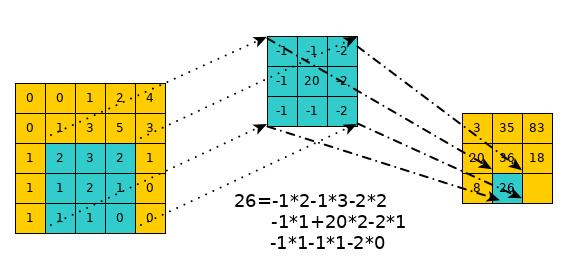
\includegraphics[scale=0.40]{conv.jpg}
\caption{Convolution layer computation}
\label{conv}
\end{figure}

The computation from a layer to another is more complex \ref{conv}.
Each layer has an internal matrix known as convolution kernel with few weights. This convolution product makes it possible to have a system invariant to translation which is particularly powerful when it comes to process images.
Convolutions aren't used alone but very often with pooling and relu layers.

\begin{figure}[!h]
\centering
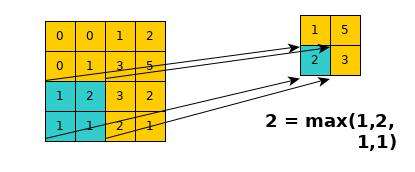
\includegraphics[scale=0.40]{pool.jpg}
\caption{Max Pooling layer computation}
\label{pool}
\end{figure}

Max Pooling layers reduce the size of the image as it goes through the network \ref{pool}.

Relu layers simply compose an activation function on the layer known as $$l_{i+1} = relu(l_i) = max(0,l_i)$$.
\subparagraph{Differences between biological vision and computer vision}

\begin{figure}[!h]
\centering
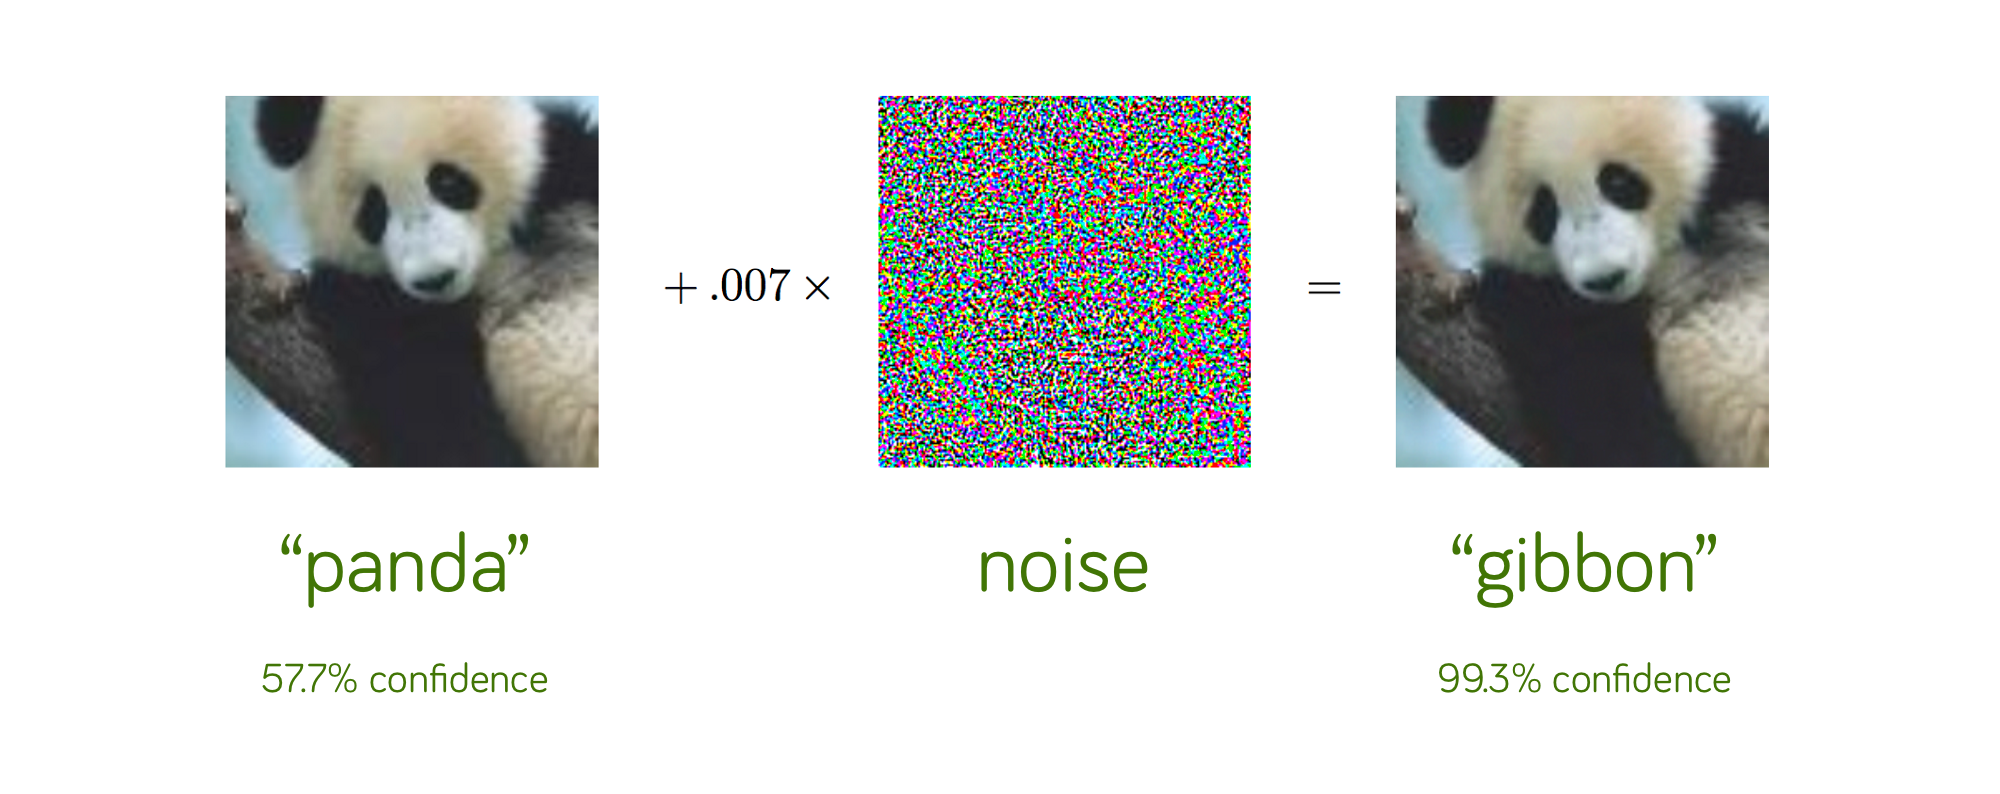
\includegraphics[scale=0.10]{adversarial.png}
\caption{Adversarial example : left - original / center - additive noise / right - adversarial example}
\label{adversarial}
\end{figure}

Convolutional neural networks tries to mimic the way brain works. However it's still a very simple model compared to the real biological computation and features which doesn't exist in human appear. The most famous feature is probably adversarial examples : classifiers may react very differently by adding small noise on images \ref{adversarial}.

Those features appear because of the difference of both systems. The main difference is probably that humans don't see the whole image at once but only small parts of them by saccading and integrating information across time to finally understand what the image represents \ref{saccades}. Thus few people tried to make a system that would replicate this behaviour by using recurrent neural network to integrate information through time and replicate this saccade system.
\subparagraph{Recurrent Neural Networks}
A recurrent neural network works similarly than a simple neural network excepts that it will keep an internal state that will interfer with next calls of the model.
\begin{equation*}
\begin{cases}
l_{i+1,t} = f_{i+1}(M_{i+1}. l_{i,t} + S_{i+1}.l_{i+1,t-1} + b_{i+1}) \\
l_{0,t} = input_t \\
l_{q,t} = output_t
\end{cases}
\end{equation*}
There is now a temporal system where computing timestep $t$ need to know the activation of the layer during the previous timestep. The first timestep is computed with an arbitrary value for the previous timestep (usually 0). This makes it possible for the network to remember previous information and to integrate information through time. Gradient descent works similarly by backpropagating through timesteps. However the network might forget rather quickly first timesteps as the training is long (high number of timesteps).

That's why there are tens of variant for the way to use the internal state such as LSTM (Long Short Term Memory) that will make it possible for the network to have a strong impact on its way to manipulate the internal state in order to control the range of the state through timesteps.
\subparagraph{Mnih \& Al Paper}
A team from deepmind has already tried to classify images with saccades in 2015 using a recurrent network being able to classify crops and to decide where to look next. They have used a very special pipeline to achieve a 99\% accuracy on MNIST (28*28 digits dataset) seeing only a set of 8*8 crops with 3 different zooms. They have used a simple neural architecture with REINFORCE to train the saccader part of the network. \ref{mnih_architecture} \cite{mnih}.
\paragraph{Objective of the project}
The aim of the project is to build a system that can learn to classify image through the saccade process we have been talking about. Mnih and Al have already done it one a small scale (MNIST) and with very simple RL algorithm. Our idea is to try to scale it with state of the art RL algorithms (PPO) and state of the art recurrent classifiers developped by the lab.
\subsection{Lab context}
For this internship I'm working with Adrien Doerig (Postdoc researcher - Internship supervisor) and Tim Kietzmann (Assistant Professor - Team supervisor). This team has been created in September 2019.
I'm working on a new project (I'm the first one with Adrien to work on it) and it will be continued for few years. My job will then be to start this project by creating tools for the next ones to work on it.
\paragraph{Global project}
The project is to use state of the art RL algorithm and convolutional and recurrent structures to train a system to classify images with saccades.
\paragraph{Internship objective}
The aim of the internship is to provide a scalable framework that will be used to go further in this project and to try, if possible, to get first results on MNIST (digits) about training both network together as well as test its resistance to adversarial attacks.

\section{Contribution}
This part will be separated into 2 subparts : first the framework I have designed and developped in order to see which tools will be used and how I've implemented them. Then we will examine different structure used to train both networks and results got for each structure.
\section{Contribution - Framework}
As the first one to actively work on the project, my job is to create a reliable framework for the next ones to work on the project to easily implement new things without worrying about learning all frameworks used to handle the RL part and the supervised part.
\subsection{GRLF - Graph Reinforcement Learning Framework}
The framework I've designed is graph based.
\paragraph{Aim of the framework}
- Easy to understand (learn and read code from others)
- Easy to extend (everyone can add code)
- Change the RL framework easily (versatile)
\paragraph{Structure of RL framework}
Most RL framework uses the same global structure with 2 very different objects : Agents and Environments.
\subparagraph{Environments}
Environments only provide observations and rewards. They are tools used by agents to learn. The most famous standard of environment is the gym envionment (made by OPENAI) which specification is fairly straighforward :
\begin{lstlisting}[language=Python]
class GymEnv:
	def __init__(self):
		#intializer
		self.observation_space = #type and shape of the observation space
		self.action_space = #type and shape of the action space
	def step(self,action):
		#modifies the state of the environment and returns obs,rew,done=(if the env needs to be reset),info=debug
		return next_observation,reward,done,info
	def reset(self):
		#resets the environment
		return initial_obs
\end{lstlisting}
This standard is widely used and all RL framework are compatible with this type of environment. Frameworks have their own environment implementation and usually standards are compiled in these standards. This means it super interesting to use the Gym standard but it's less powerfull than internal environment data structures.
\subparagraph{Agents}
In most RL framework agents have the main loop during the training. It will call the environment to build trajectories. There isn't any standard for agents which means we will need to be particularly carefull to this so that every agent system from a new framework would still be compatible.
\paragraph{Structure of the framework}
\subparagraph{General system}
To be sure to be compatible it's important to keep the agent/environment system. The framework must makes it possible for the user to define a system that will be compiled in an agent/environment system to call libraries accordingly. This way the user doesn't need to understand how RL framworks function in depth to build its system.
\subparagraph{Graph dynamics}
The main idea is to propose an interface based on a graph which will be defined by the user describing the dynamics of the system \ref{graph_dynamics}. This graph will be composed of modules (nodes) that will be connected between each other.
\subparagraph{Modules}
A module is an object that can be connected to other modules through its \emph{ports} (analogy with networks). A \emph{port} is a value from a module that can be accessed from other modules and shared with them. Basically a module gets information from other modules through its ports, computes something with this values and  store outputs of the computation in its ports to be sent to other modules. Thus the following architecture will be used :
\begin{lstlisting}[language=Python]
class Module:
	def __init__(self):
		#intializer
	def run(self):
		#Compute things
\end{lstlisting}
Ports are defined using python objects as dictionaries : 3 prefix keys will be used to interact with ports :
\begin{itemize}
\item '*' : define a port and give its type
\item ':' : redefine the type
\item '$\epsilon$' : get the value of the port
\item '>' : used to create links between node (we will get back to it later)
\end{itemize}
Here is an example of the definition of a module :
\begin{lstlisting}[language=Python]
class DoubleModule:
	def __init__(self):
		#intializer
		self["*a"] = float #definition of port a as float
		self["*b"] = float #definition of port b as float
	def run(self):
		#Compute things
		self["b"] = self["a"]*2 #Use the value of port a to double it and put it in port b
d = DoubleModule()
print(d["a"])
>>> None
d["a"] = 5.
d.run()
print(d["b"])
>>> 10.
d[":a"] = int #Will autoconvert the initial value in a to int
d.run()
>>> Exception : port b has type float but received int value
d[":b"] = object #Universal type
d.run()
print(d["b"])
>>> 10
\end{lstlisting}
As you can see I've added a type system that doesn't exist in Python to make it more convenient for users. It's possible to bypass it if needed. Several modules can be defined this way to compute complex functions.
\subparagraph{Connecting modules}
Modules can be connected with the following syntax :
\begin{lstlisting}[language=Python]
#Define module 1
module1 = Module()
module1["*a"] = int
#Define module 2
module2 = Module()
module2["*a"] = int
#Connect module1["a"] to module2["a"] (-> direction of arrows)
module1[">a"]([module2[">a"]])
\end{lstlisting}
\subparagraph{Loop and Graph object}
Loop makes it possible to handle the system we have talked about to compute modules and ports dynamics :
\begin{lstlisting}[language=Python]
#Define module 1
loop = Loop([module1,module2],nb=1) #Modules will run in this order (nb=1 iteration of the loop)
module1["a"] = 5
print(module2["a"])
>>> None
loop.run() #run module1.run (empty) then send module1["a"] to module2["a"] and run module2.run() (empty)
print(module2["a"])
>>> 5
\end{lstlisting}
With this loop system it's possible to run a sequence of modules several times.
\subparagraph{Graph and agent/environment system}
Graph object makes it possible to compute the agent/environment system. First we need to define an RL\_Module :
\begin{lstlisting}[language=Python]
import tensorflow as tf #Main ML library -> tf.Tensor is an array
class RL_Module(Module):
	def __init__(self,input_shape,output_shape):
		self["*input"] = (tf.Tensor,input_shape) #Observation : type and shape
		self["*output"] = (tf.Tensor,output_shape) #Action : type and shape
		self["*reward"] = (tf.Tensor,(None,1)) #Reward : type and shape
	def run(self):
		#Compute things
\end{lstlisting}
Once a RL\_Module is defined in a Loop object it can be upgraded to a Graph object in order to get the agent/environment system. This is a dummy example with empty modules to show how it works :
\begin{lstlisting}[language=Python]
#Definition of Modules (nodes)
rl_module = RL_Module((10,),(2,))
m1 = Module()
m1["*action"] = tf.Tensor
m1["*a"] = tf.Tensor
m2 = Module()
m2["*a"] = tf.Tensor
m2["*obs"] = tf.Tensor
m2["*reward"] = tf.Tensor
#Definition of connections
rl_module[">output"]([m1[">action"]])
m1[">a"]([m1[">a"]])
m2[">obs"]([rl_module[">input"]])
m2[">reward"]([rl_module[">reward"]])
#Definition of the graph
loop = Loop([m1,m2,rl_module],nb=10) #Run 10 times the list
graph = Graph(loop)
#Run the graph
print(graph.environment)
>>> GymEnv at XXXXXXXX
print(graph.agent)
>>> Agent at XXXXXXXX
graph.run(1000) #Run 1000 times the loop
\end{lstlisting}
It's then possible to only use the agent or the environment from the graph object with an other framework if needed. The agent is compatible with GymEnvironments and the environement is a GymEnvironment. You can also run both together with the graph.run method. We'll now see how to implement RL\_Modules more in depth to then go further in difficulties of implementation.
\subparagraph{RL\_Modules more in depth}
In the team we aren't professional of RL which means we will prioritize using existing powerfull RL framework in order to be sure about the effectiveness and efficiency of the implementation of the algorithm. Thus in most RL frameworks, agents are objects with a run method and an environment parameter. Calling this method will run the main training loop. However in GRLF the definition of the graph contains both the agent and the environment with a loop system including both. This means it's won't be easy to switch from this data structure to the other.

To transform this data structure to the desired one, the RL\_Module.run method will throw an exception when called. This makes it possible for the loop.run method to behave like the environment would. The exception will contain inputs for the RL framework \ref{grlf_trick}.

Thus we have added a new method for modules : the run\_after method that will be called right after the run method. Now the RL\_Modules code looks like that :
\begin{lstlisting}[language=Python]
import tensorflow as tf #Main ML library -> tf.Tensor is an array
class RL_Module(Module):
	def __init__(self,input_shape,output_shape):
		self["*input"] = (tf.Tensor,input_shape) #Observation : type and shape
		self["*output"] = (tf.Tensor,output_shape) #Action : type and shape
		self["*reward"] = (tf.Tensor,(None,1)) #Reward : type and shape
		self.learn_fn = #Function from the RL framework : (env,nb_timesteps) -> object
	def run(self):
		#Compute things
		raise RLInput(self["input"]) #raises the exception
	def run_after(self):
		#Compute things with self["output"] = output of the agent in the RL framework
\end{lstlisting}
\paragraph{Advanced modules used}
There are several objects modules can heritate from (which creates a type system over modules) : FitableModules (contains a datastructure that can learn) and PointerModules.
\subparagraph{MNIST Database}
This module doesn't have any port used as input. It will fill its "img" port with a MNIST image and the "label" port with its label. Images and labels are changed each time the run method is called. Images are chosen in the order of the database (n call is the n-th image of the dataset).

\subparagraph{Cropper}
This module is very simple : it gets as input an image "img" and crop coordinates "x","y" and the run method will return in "output" the smaller image corresponding to "img" cropped at those coordinates.

\subparagraph{ModelModule - FitableModule}
A ModelModule has an internal neural network and two ports : "input", "output". Calling run calls the network on "input" and returns the result in "output". The user can also access any layer in the neural network through the port that has the same name.

\subparagraph{Classifier - PointerModule FitableModule}
A Classifier module is a PointerModule to a FitableModule and will have 4 ports : a reshaped "output", a "label" port for the real label, a "plabel" port for the predicted label and a "issue" port with a boolean value about whether the predicted label is the same as the real label. Calling run will call the ModelModule run method, reshape the output to a given shape (it's more convenient this way), computes the predicted label from the output of the neural network to then fill the "issue" port.

\subparagraph{BatchCapsule - PointerModule}
This pointer module is more complex : it will capture each input in "input" and "label" ports of the pointed module and store them in a batch. Once enough data collected (treshold defined by the user) it will fit the pointed module on collected data (it should point to a FitableModule).

\subparagraph{PPOSaccader - PointerModule,FitableModule}
A RL\_Module with a learn\_fn for PPO which points toward a FitableModule. It will compute x and y coordinates for the saccade from the output of its FitableModule.

During the internship we have tried 2 different RL frameworks for PPO : OPENAI baselines (tf-2 branch), the original PPO from its creators and RLLib which is scalable on multi gpu clusters.
\begin{itemize}
\item The OPENAI framework uses a learn function to train the agent on the given environment which means it will be very easy to implement its RL\_Module.
\item RLLib is more complex and we need to define the policy with the associated PPO loss (easily modifiable) to get our agent. The learn function is then a custom learn function that will use RLLib system to train the agent.
\end{itemize}
\section{Contribution - Structure of the system}
Now that we have seen the framework which will be used, let's talk about the structure for the classification system.

At first we have used this graph \ref{base_graph} with OPENAI baselines. This means the GRLF framework will generate the environment/agent system. When the training will start, the environment.reset method will be called running the loop until an exception is thrown by the RL\_Module which means it will load an image, crop it and feed it to the RL framework. Then each time environment.step is called, it will run then end of the loop, loop back and reload an other image. It will loop loop.nb times until its next reset (gymEnv.step returns done=True).
\subsection{Two different networks}
Here we have 2 independant networks : the classifier and the saccader. We thought it would relevant to separe both and to train them independently because the first one will learn with supervised data when the other one will learn with reinforcement learning. The main issue with crossing them into one single network is that the RL training contains much more noise than supervised learning (it takes time to fully understand such a vast environment). Thus if the network share layers the gradient of the RL part might interfere with the classifier network and its noise might reduce the efficiency of the training.

We have tried at first a feed forward version of the system which means the classifier isn't recurrent : it needs to classify the image using a single crop. However it will still have several saccades for the saccader to find the best crop to give to the classifier to be sure about its prediction. This system is shallow which means its easier to debug than a full recurrent system.

To test the pipeline properly we have used 3 different environments : 
\begin{itemize}
\item 2 spots environments - 2 possible crops : centered and left. This is a very basic environment (discrete action space) which is made for the agent to focus on the centered crop. The left one is too far to see the digit properly which means it's a suboptimal crop and the centered one should be prefered.
\item 5x5 environment - This environment is an evolution of the previous one. It's still a discrete action space which simplifies the system but it's more complex : a 5x5 grid makes it possible to have much more reliable fixations.
\item Continuous environment - It's the complete version of the environment.
\end{itemize}

Once the feed forward system works fine we have worked on the recurrent one. To test the pipeline and start working on recurrent networks we have started with LSTMs.



\subsection{A branch network}
An other idea we have tried especially because of technical problem is to follow Mnih \& Al intuition : one network with 2 outputs and 2 way to learn. 


\section{Difficulties}
\subsection{Architecture of the framework}
This internship was very technical especially about the coding part. I have spent a lot of time thinking about the architecture for the framework in order the have something easy to use, efficient (it's python which means it crucial to think about execution time) and versatile.
\subsection{Documentation of RL frameworks}
RL frameworks we have used are recent which means the documentation is very soft and it's often hard to find why your program doesn't work with information found in the documentation or on the internet. To understand how to implement such an innovative and original system I had to read the source code of huge libraries to produce a small code that would actually work fine. This lack of documentation was a real issue and I've spent most of my time reading and printing everything in RL frameworks to really understand how to hack those framework into our original system.
\subsection{Chaotic aspect of the system}
This classifier + saccader system is very unstable : let's assume the saccader one saccades on the top left hand corner. The classifier will only get crops from this fixation. This means it will fit on top left centered crops and won't develop knowledge about the rest of image space. If it only sees the top left part of digits when it sees an other crop it won't understand it and won't be able to classify it. This way when the saccader explores, crops won't be understood by the classifier which will result in low rewards. Thus the system will be stuck on the top left spot and won't move anymore event if this spot isn't optimal. This means the function that is minimized through this process has a lot of local minima and the starting point and the way optimization is done are crucial. This makes the system very unstable which is akward because usually supervised learning of classifiers is very reliable.
\section{Conclusion}
COMING SOON :)
\end{document}
